\documentclass[11pt]{article}\usepackage[]{graphicx}\usepackage[]{color}
%% maxwidth is the original width if it is less than linewidth
%% otherwise use linewidth (to make sure the graphics do not exceed the margin)
\makeatletter
\def\maxwidth{ %
  \ifdim\Gin@nat@width>\linewidth
    \linewidth
  \else
    \Gin@nat@width
  \fi
}
\makeatother

\definecolor{fgcolor}{rgb}{0.345, 0.345, 0.345}
\newcommand{\hlnum}[1]{\textcolor[rgb]{0.686,0.059,0.569}{#1}}%
\newcommand{\hlstr}[1]{\textcolor[rgb]{0.192,0.494,0.8}{#1}}%
\newcommand{\hlcom}[1]{\textcolor[rgb]{0.678,0.584,0.686}{\textit{#1}}}%
\newcommand{\hlopt}[1]{\textcolor[rgb]{0,0,0}{#1}}%
\newcommand{\hlstd}[1]{\textcolor[rgb]{0.345,0.345,0.345}{#1}}%
\newcommand{\hlkwa}[1]{\textcolor[rgb]{0.161,0.373,0.58}{\textbf{#1}}}%
\newcommand{\hlkwb}[1]{\textcolor[rgb]{0.69,0.353,0.396}{#1}}%
\newcommand{\hlkwc}[1]{\textcolor[rgb]{0.333,0.667,0.333}{#1}}%
\newcommand{\hlkwd}[1]{\textcolor[rgb]{0.737,0.353,0.396}{\textbf{#1}}}%
\let\hlipl\hlkwb

\usepackage{framed}
\makeatletter
\newenvironment{kframe}{%
 \def\at@end@of@kframe{}%
 \ifinner\ifhmode%
  \def\at@end@of@kframe{\end{minipage}}%
  \begin{minipage}{\columnwidth}%
 \fi\fi%
 \def\FrameCommand##1{\hskip\@totalleftmargin \hskip-\fboxsep
 \colorbox{shadecolor}{##1}\hskip-\fboxsep
     % There is no \\@totalrightmargin, so:
     \hskip-\linewidth \hskip-\@totalleftmargin \hskip\columnwidth}%
 \MakeFramed {\advance\hsize-\width
   \@totalleftmargin\z@ \linewidth\hsize
   \@setminipage}}%
 {\par\unskip\endMakeFramed%
 \at@end@of@kframe}
\makeatother

\definecolor{shadecolor}{rgb}{.97, .97, .97}
\definecolor{messagecolor}{rgb}{0, 0, 0}
\definecolor{warningcolor}{rgb}{1, 0, 1}
\definecolor{errorcolor}{rgb}{1, 0, 0}
\newenvironment{knitrout}{}{} % an empty environment to be redefined in TeX

\usepackage{alltt}
\usepackage{fullpage}
\usepackage{amsthm,amsmath,amsfonts,amsbsy,graphicx,calrsfs,amssymb}
\usepackage{latexsym,graphicx}
\usepackage{amsfonts}
\usepackage[toc,page]{appendix}
\usepackage{setspace}
\usepackage{titlesec}
\usepackage{float}

\setlength\parindent{0pt}
\IfFileExists{upquote.sty}{\usepackage{upquote}}{}
\begin{document}
\begin{center}
\textbf{NYCC 2015-2018 Arrest Analysis}\\
\normalsize{James Wu}
\end{center}

\section{Introduction}
The NYC Council's Public Safety Committee has asked the Data team for an analysis of arrests from 2015-2018. They want to know about whether arrest rates have decreased and overall trends in arrests during this period. Based on this and the districts of interest, the questions we will explore in this report are as follows:
\begin{itemize}
  \item \textbf{Has the arrest rate been decreasing from 2015-2018}
  \item \textbf{What are the top 5 most frequent arrests types in 2018?}
  \item \textbf{How has the overall trends of arrest types changed from 2015-2018?}
  \item \textbf{Is there more crime (assuming arrests is a sample of total crime) in precinct 19 (Upper West Side) than in precinct 73 (Brownsville)? What are the trends?}
\end{itemize}
\\

\section{Data}
We are using NYPD Arrests Dataset available at \emph{https://data.cityofnewyork.us/Public-Safety/NYPD-Arrests-Data-Historic-/8h9b-rp9u} for this study. The data is manually extracted every quarter and reviewed by the Office of Management Analysis and Planning before being posted on the NYPD website. Each record in this dataset represents an arrest effected in NYC by the NYPD and includes information about the type of crime, the location and time of enforcement, and the arrestee's demographic. As the dataset has records from 2006, we used only a subset of the data, including only 2015-2018 records. This data was reviewed for consistency and expected patterns, then prepared (i.e. formatting, creating new variables) for the study. Three new numerical columns were generated from the \textit{ARREST\_DATE} column: \textit{ARREST\_YEAR}, \textit{ARREST\_MONTH}, and \textit{ARREST\_DAY}.

\section{Methodology}
All data preparation and analyses were conducted in R. In deciding appropriate models to answer the questions, we first explored how the data looked like with daily, monthly, and annual aggregated counts. We saw similar patterns in all three aggregations.
\\\\
One particular property of the data is its time-element. When looking at the aggregated monthly arrest plots, the data seems to display signs of having a seasonal pattern. Every start of the year has a spike in arrests in January, followed by a sharp decline in February. There are usually higher arrests in March, May, and August following lower arrests in February, April, and July (Figure: \ref{fig:monthlyArrests}). The seasonality could be potentially explained by: (1) there may be less or more cops deployed for certain months due to holidays, or annual events, (2) people's behaviors may also be influenced by seasons, temperatures, holidays, etc. (3) the cyclical nature of new hires and people leaving, and other potential reasons. 
\\\\
Since we are concerned about overall trends, yearly aggregated data is primarily used for our linear models to reduce the effects of omitted variable bias and to remove seasonality. Monthly aggregated data was used for data exploration purposes, and daily aggregated data was largely unused due to high noise.  If seasonality is removed, the independence assumption for linear regressions is more believable.

\section{Analysis and Results}
\subsection{Arrest rate trends}
We found the general trend of arrests has been steadily decreasing from 2015-2018. There were 339,470 arrests in 2015, dropping to 246,773 arrests in 2018, a 27\% drop.
\\\\
To quantify this trend, we used a linear regression model on the aggregated yearly data removing seasonality. The specified model is: $CRIME\_COUNT=\beta_0+\beta_1YEAR$. We found \textit{YEAR} variable to be statistically signicant at an alpha of .05, and with a negative coefficient which signifies a downwards trend. On average, the number of arrests have decreased by 30,673 per year on our fitted trend line (Figure: \ref{fig:Yearlytrend}).

\subsection{Evolution of the top 5 arrest reasons}
The top 5 arrest reasons in 2018 were 3rd degree assault, petit larceny, traffic misdemeanor, 2nd degree assault, and 7th degree possession of controlled substances in that order. In contrast, the top 5 arrest reasons in 2015 were theft of services, 3rd degree assault, petit larceny, 7th degree possession of controlled substances, and unclassified NYS laws in that order.
\\\\
Theft arrests has decreased 76\% over the years, and arrests under "unclassified NYS laws" has decreased by 94\% (Although, I suspect this may be because this classification may have been spread out to other offenses). 3rd degree assault, petit larceny, 2nd degree assault, and unclassified traffic misdemeanors have had relatively stable number of arrests throughout the years. Refer to Figure: \ref{fig:crimeOverYears} in the Appendix for more details.

\subsection{Precinct 19 vs. precinct 73}
If we assume that arrests is a sample of total crime, we found that precinct 73 (Brownsville) had a much higher crime than in precinct 19 (Upper East Side) with also a much larger variance month to month (Figure: \ref{fig:BrownUES}). However, while arrests have been decreasing at a fast rate in Brownsville, arrest counts in the Upper East side have been relative stable from 2015-2018. 
\\\\
To quantify this trend, we used a linear regression model on the aggregated yearly data removing seasonality. The specified model is: $CRIME\_COUNT = \beta_0 + \beta_1YEAR + \beta_2PRECINCT73 +\beta_4YEAR*PRECINCT73$, where \textit{PRECINCT73} is a indicator for whether it is Brownsville or not. We found that Brownsville has on average 2,143,694.1 - 1,060.90 * \textit{YEAR} more crime than Upper East Side; so in 2016, Brownsville had on average 4,920 more crime (2,143,694.1 - 1,060.90 * 2016). This also tells us that while both Brownsville and Upper East side has a decreasing trend (negative slopes), Brownsville's arrest count was decreasing on average 1,060.90 more than Upper East Side's decreasing trend of 147.9 per year (Figure: \ref{fig:BrownUEStrend}).

\section{Future Work - Predictive Modelling}
To optimize NYC's police resources, we could potentially build a predictive model based on past arrests to predict the likelihood of a crime happening in any district. A logistic regression with added seasonality terms can be used for this.
\\\\
The difficulty of this task could be the construction of the classifier. There are usually at least 1 arrest daily, so a binary term indicating whether an arrest was made in a day would not be particularly useful (ie. 100\% every day, every where!) A solution for this could be creating subjective cutoff point(s) (e.g. high crime/medium crime/low crime) for the classifier. 
\\\\
There is also the problem of the ethics in equating arrests with crime. We run the risk of perpetuating prior biases due either historic bias or a change of law (e.g. marijuana decriminalization). We can reduce the probability of happening by excluding sensitive demographic data. All variables could be included in the model, excluding the repeat ones such as code and its description (choose one to avoid multicollinearity), \textit{ARREST\_KEY}, and \textit{PERP\_RACE}.
\\\\
Our model may be evaluated by using a certain time-frame as the training data, such as 2015-2017, and another outside the timeframe as test data, like 2018. We can look the model's accuracy and mis-classification rate.

\newpage

\section{Appendix}

\begin{figure}[H]
  \centering
    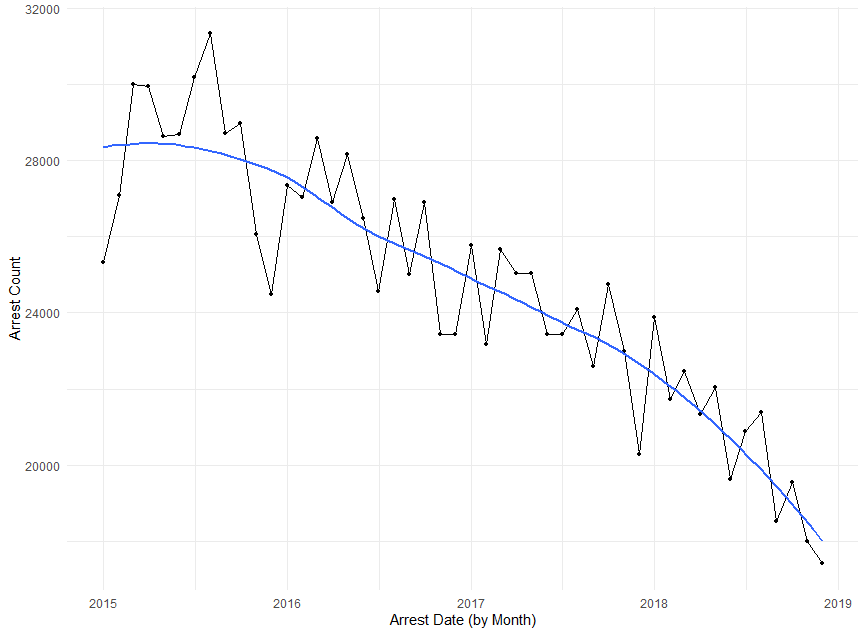
\includegraphics[width=0.65\textwidth]{monthlyArrests.png}
  \caption{\textbf{NYPD Monthly Arrests.} There appears to be some seasonality shown annually.}
  \label{fig:monthlyArrests}
\end{figure}

\begin{figure}[H]
  \centering
    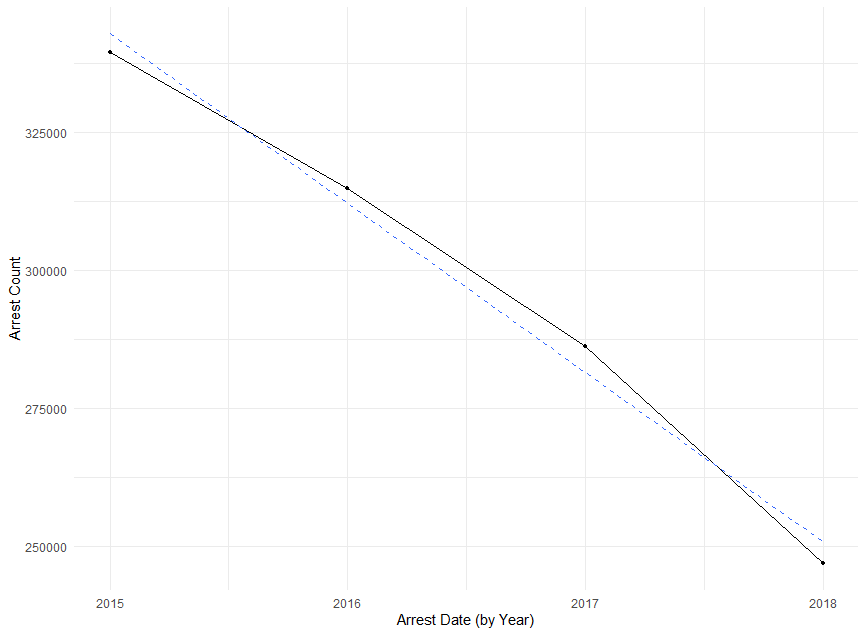
\includegraphics[width=0.65\textwidth]{Yearlytrend.png}
  \caption{\textbf{Linear Regression on Annually Aggregated Data.}}
  \label{fig:Yearlytrend}
\end{figure}

\begin{figure}[H]
  \centering
    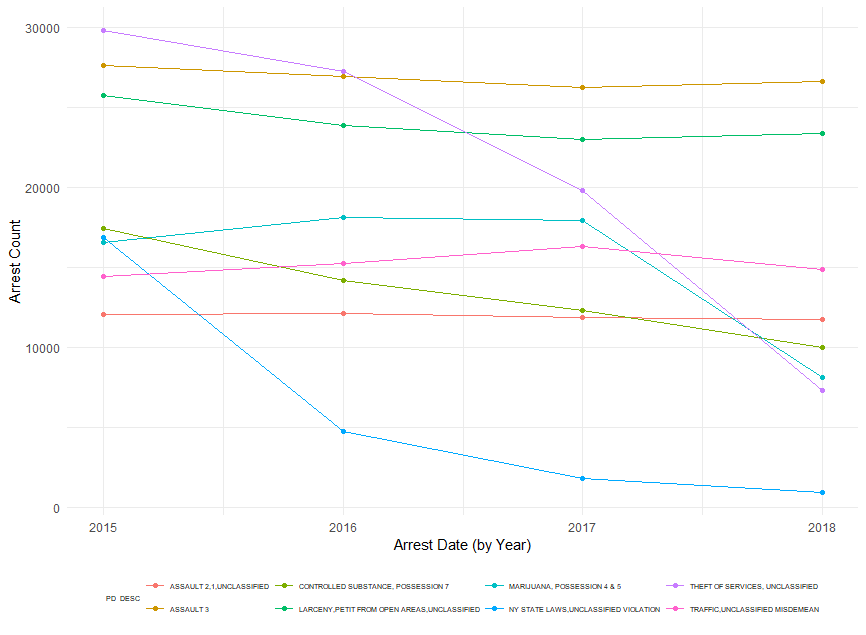
\includegraphics[width=0.65\textwidth]{crimeOverYears.png}
  \caption{\textbf{Evolution of Arrest Types from 2015-2018.}}
  \label{fig:crimeOverYears}
\end{figure}

\begin{figure}[H]
  \centering
    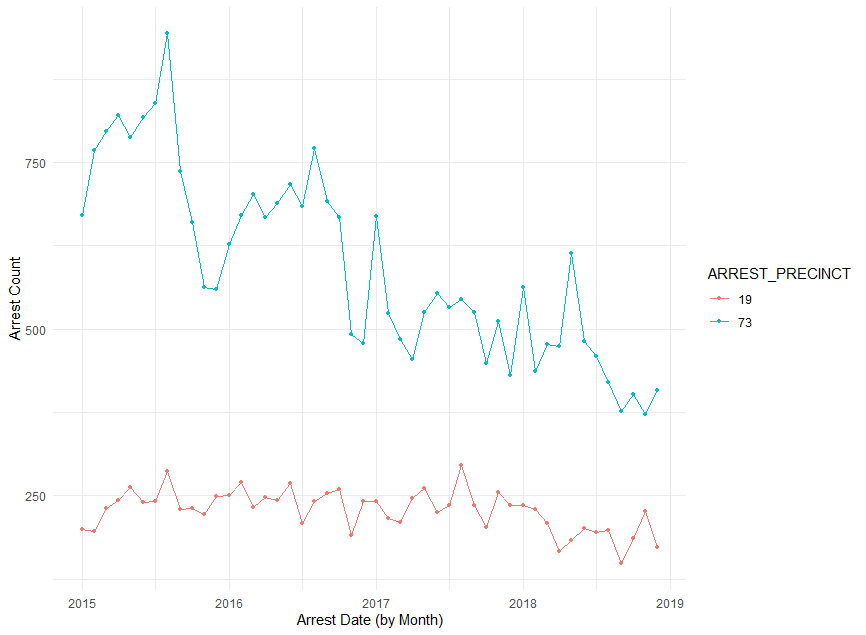
\includegraphics[width=0.65\textwidth]{BrownUES.png}
  \caption{\textbf{Monthly crimes in Brownsville (precinct 73) vs. Upper East Side (precinct 19).} Brownsville has a larger variance per month, depicted by large jumps.}
  \label{fig:BrownUES}
\end{figure}

\begin{figure}[H]
  \centering
    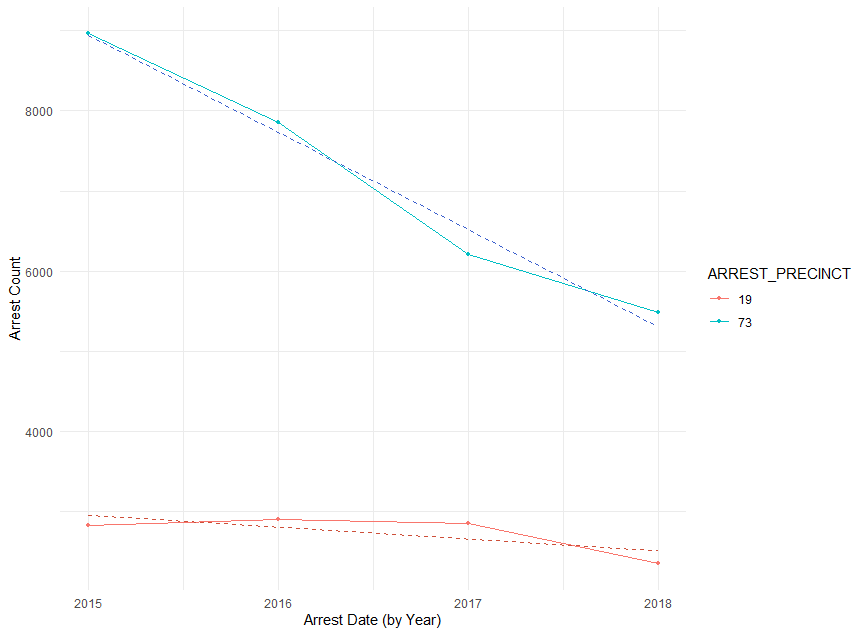
\includegraphics[width=0.65\textwidth]{BrownUEStrend.png}
  \caption{\textbf{Linear Regression on Annually Aggregated Data for Precinct 73 and Precinct 19.}}
  \label{fig:BrownUEStrend}
\end{figure}

\end{document}
